\subsection{Long Context}
\label{subsec:lc}

The Nemotron 3 models are designed to support context lengths up to 1M tokens to enable extended multi-turn agentic reasoning. Rotary Position Embeddings (RoPE) are a known hurdle to extending context beyond the training length. Since Mamba layers provide implicit positional information, Nemotron 3 models do not use RoPE in attention layers and therefore do not suffer from out-of-distribution RoPE issues during context extension (a Transformer analog is explored in \cite{puvvada-etal-2025-swan}). For \ourmodel, we included a continued pre-training (CPT) stage at a 512k sequence length, and supervised fine-tuning (SFT) was performed at a 256k sequence length. In addition, we include a long-context environment in the reinforcement learning stage with inputs up to 32k tokens. All three stages included synthetic data designed to support long-range retrieval, multi-hop reasoning, multi-document information aggregation, and related capabilities. In CPT, we did not observe the need to follow a staged increase of training sequence length from 8k to 512k. Further, we observe that the MoE hybrid architecture adopted for the Nemotron 3 models has better context extension capability compared to the dense hybrid architecture used in Nemotron 2 Nano. When continue pre-trained on the same sequence length (512k), the Nemotron 3 Nano base model shows better RULER \citep{hsieh2024ruler} scores compared to the Nemotron 2 Nano 12B base model at a 1M context length (Table \ref{tab:base_ruler}).

To further assess how well Nemotron 3 Nano leverages very long contexts for next-token prediction, we measure the negative log-likelihood (NLL) of tokens at various positions in held-out sequences. Lower NLL indicates better predictive performance. In a related coherent sequence, tokens appearing later in the context should be easier to predict and therefore exhibit lower NLL. We conduct this analysis on repository-level code sequences larger than 1 million tokens. Figure \ref{fig:nano_v3_base_nll} shows the cumulative average NLL up to each token index for \ourmodel base. We observe that NLL decreases with sequence length, suggesting that the model is able to use long input context up to the tested range.

\begin{table*}[h]
\centering
\begin{tabular}{l|cccc}
\toprule
\textbf{Model} & \textbf{128k} & \textbf{256k} & \textbf{512k} & \textbf{1M} \\
\midrule
Nemotron-Nano-12B-v2-Base & 85.13 & 79.85 & 75.12 & 23.43  \\
\ourbasemodel & 74.48 & 71.67 & 66.02 & \textbf{54.19}  \\
\bottomrule
\end{tabular}
\caption{RULER scores for Nemotron-Nano-12B-v2-Base (Dense  Hybrid) and \ourbasemodel (MoE hybrid) models at different input context lengths. We observe that MoE hybrid model is more robust to length extrapolation than dense Hybrid Model. Nemotron-Nano-12B-v2-Base model shows abrupt dropoff between 512k and 1M, where as \ourbasemodel exhibits graceful degradation. Both models were trained upto 512k sequence length.}
\label{tab:base_ruler}
\end{table*}

\begin{figure}[h]
    \centering
    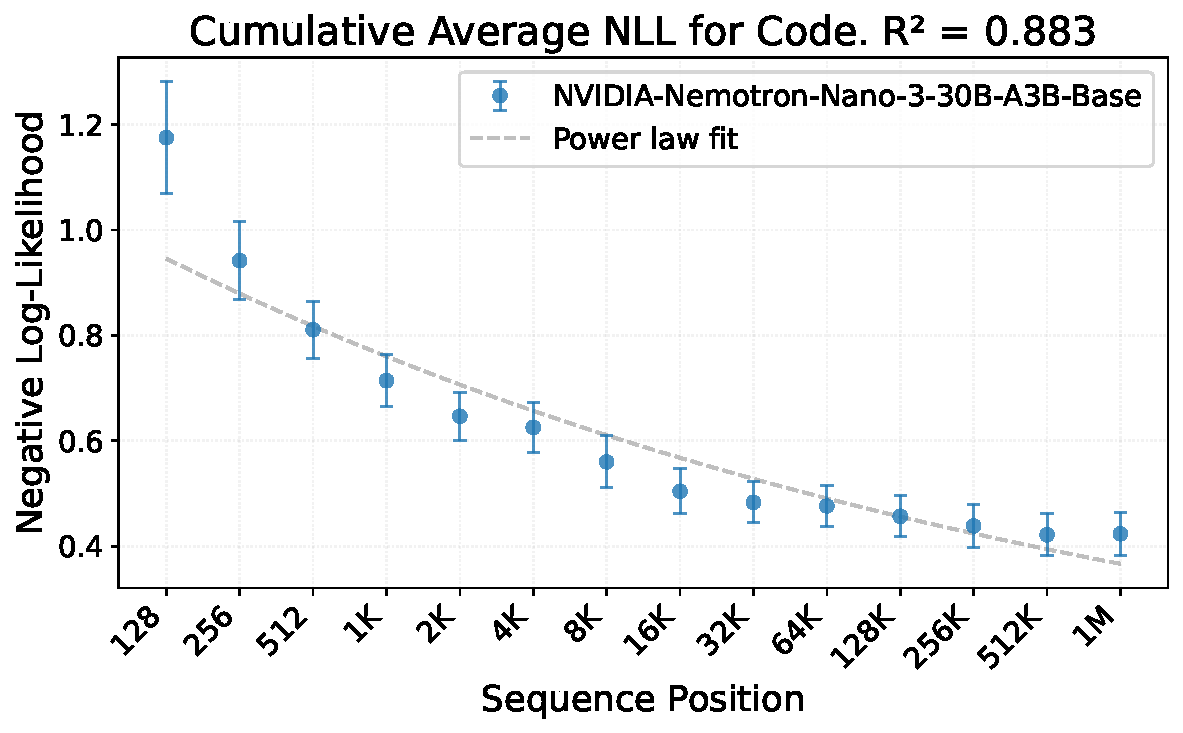
\includegraphics[width=0.5\linewidth]{figures/nanov3_base_code.pdf}
    \caption{Cumulative average Negative loglikelihood (NLL) as a function of token position in code data. \ourmodel base shows improved predictions upto 1M tokens in code data. 
    }
    \label{fig:nano_v3_base_nll}
\end{figure}
